\documentclass{article}
\usepackage[utf8]{inputenc}
\usepackage[margin=0.5in]{geometry}
\usepackage{datetime2}
\usepackage{bytefield}
\usepackage{algorithm,algpseudocode}
\usepackage{amsmath,amsfonts}
\usepackage{xcolor}
\usepackage{makecell}
\usepackage{graphicx}
\setlength{\parindent}{0pt}


\title{CSE 475 Creature Spec}
\author{Ryan Rowe, Austin Beaulieu}
\date{Rev. \today~\DTMcurrenttime}

\newcommand\ind[1]{\ensuremath{[\![#1]\!]}}
\newcommand\code{\texttt}
\newcommand\hex[1]{\texttt{0x#1}}
\newcommand\bin[1]{\texttt{0b#1}}
\newcommand\uint[1]{\code{uint#1\_t}~}
\newcommand\sint[1]{\code{int#1\_t}~}
\newcommand\float{\code{float}~}
\newcommand\assign{\ensuremath{\leftarrow}~}
\newcommand\rand{\text{rand}}
\newcommand\todo[1]{\textcolor{red}{TODO: #1}}

\begin{document}

\maketitle

\section{Summary}
\qquad {\large In this capstone we will function as a single mega-design team who have been commissioned to design and program a multi-nodal mesh radio-controlled set of ``Creatures'' who live in a large public space such as the Allen Center Atrium. The ``Creatures'' make sound, emit multi-colored light, sense motion, sense light levels and noise levels, and communicate to each other through 900MHz packet radio transmissions.}\\

\qquad {\large All ``Creatures'' obey a common set of rules of behavior, which encourages cooperation between ``Creatures'' and cumulatively produce emergent behavior of the group. This effect should be pleasing and relaxing, much more beneficial and entertaining than the usual background music.}\\

\qquad {\large We will explore such technologies as mesh networking, interrupt-driven multi-threaded processing, power-saving techniques, and rule-making to achieve leaderless emergent behavior. We will apply non-technical skills such as selecting colors and patterns and sounds for their expressive, evocative, and pleasing aesthetic effects.}\\

\begin{centering}
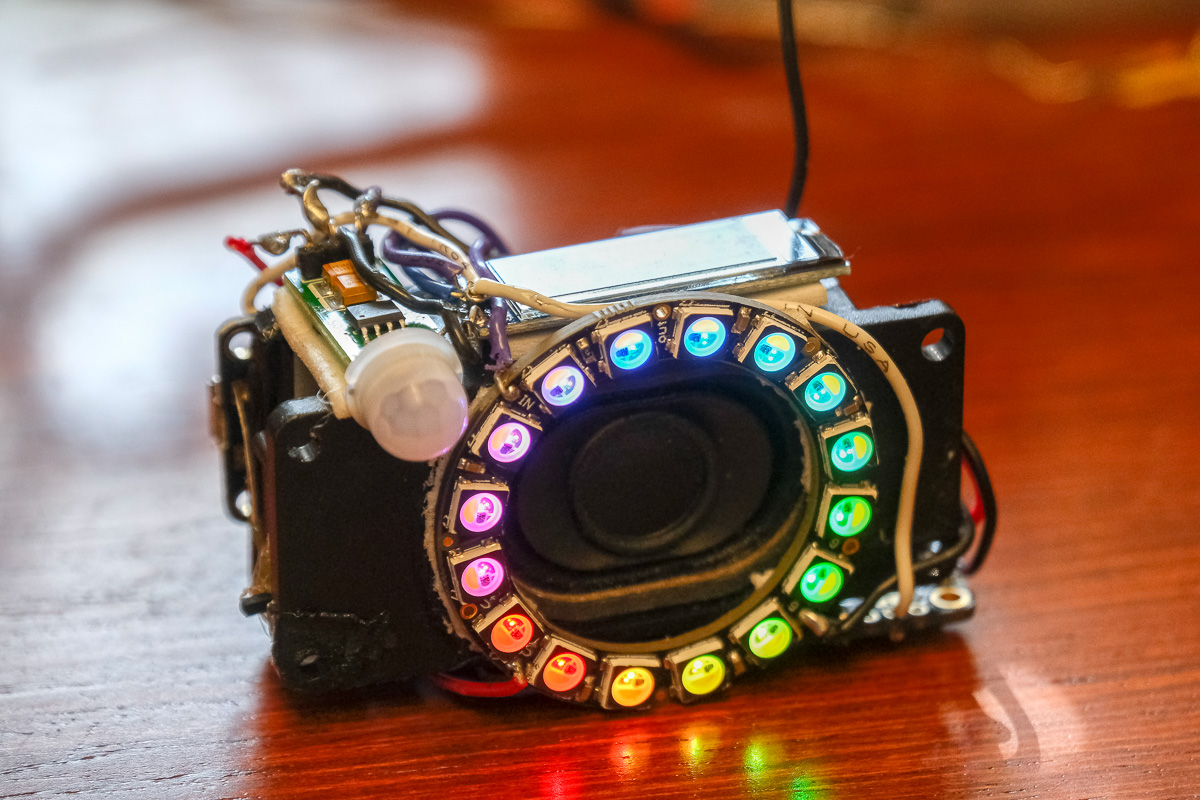
\includegraphics[width=16cm]{images/creature}
\end{centering}

\clearpage
\section{The Creature Algorithm}

\subsection{Initialization}
When each creature turns on, it must go through initialization:

\begin{enumerate}
    \item Wait for communication with Controller
    \item Receive \& set data from AdjustGlobals packet
    \item Initialize current state randomly from the list of standard states
\end{enumerate}

\subsection{Loop}
For every \code{RepeatCycle} amount of time, run the following process:
\begin{enumerate}
    \item If the controller sends PlaySound(N) or PlayEffect(N), play that sound and/or effect, else play current state
    \item Start the radio and set listen timer for $\rand(\code{minListen}, \code{maxListen})$ milliseconds for other creatures and/or the controller
    \item Calculate the transition to the next state
    \item Set a timer for \code{minListen} for sending the new state to other creatures when timer fired
\end{enumerate}


\subsection{Bookkeeping}
Each creature needs to maintain values pertaining to the global state of the creature network and to the internal state of the creature itself. This section outlines these values.

\subsubsection{Global Values}
Creatures will receive state transition packets from other creatures. Each should maintain a list of the states other creatures are in and update this as it changes. We refer to this as the \code{StateList}. If a creature has not contacted another, they should assume it to be in the wait state (\hex{00}) internally. The creature should also maintain a running average of RSSI from these packets. This average should serve as a reasonably accurate heuristic for the distances from other creatures. We refer to this as \code{DistanceList}.

\subsubsection{Local Values}
Several values must be maintained by the program pertinent to the creature itself. These values are used for computing state transitions \& startles.\\

\begin{tabular}{l|l}
    \textbf{Variable} & \textbf{Description} \\\hline
    \uint{32} \code{LAST\_STARTLE} & Time in milliseconds since last startle\\
    \uint{8} \code{LAST\_STARTLE\_ID} & The last startle ID received\\
    \uint{8} \code{STARTLE\_THRESHOLD} & Current numeric value of the startle threshold\\
    \code{State} \code{CURRENT\_STATE} & The current state object being maintained\\
    \uint{8} \code{REPEAT\_STATE} & How many more state repetitions before calculating the next state\\
\end{tabular}

\clearpage
\section{Packet Protocol}

Packets are sent and received in the following format. The first byte is the packet identifier, followed by the originating address (either $2\times\mbox{kit}$ or $2\times\mbox{kit} - 1$) and destination address. To send a packet to all creatures, use the broadcast address \hex{FF}.\\

\begin{bytefield}[bitwidth=\textwidth/48]{48}
\bitheader{0-24}\\
\bitbox{8}{\uint{8} \code{pid}}
\bitbox{8}{\uint{8} \code{src\_addr}}
\bitbox{8}{\uint{8} \code{destAddr}}
\bitbox{24}{\uint{8} \code{payload[sizeof(packet) - 3]}}
\end{bytefield}

All payload contents are listed by their byte offset inside the payload array.

\subsection{Broadcast Packets}
These are all packets that are broadcast by the controller to your creature. You should verify that \code{src\_addr == 0} and \code{dst\_addr} is either your creature's address or the broadcast address.

\begingroup
\renewcommand{\thesubsubsection}{PID \hex{\ifnum\value{subsubsection}<10 0\fi\arabic{subsubsection}}}
\setcounter{subsubsection}{-1}

\subsubsection{Set Globals}

Updates a series of creature variables. Only valid if \code{src\_addr == 0}.\\

\begin{tabular}{r|l|l|l}
\textbf{Byte} & \textbf{Variable} & \textbf{Default} & \textbf{Description}\\\hline
0 & \uint{16} \code{TX\_POWER} & 1 & Radio transmit power\\
2 & \uint{8} \code{STARTLE\_RAND\_MIN} & 100 & Minimum bound when generating startle strength\\
3 & \uint{8} \code{STARTLE\_RAND\_MAX} & 200 & Maximum bound when generating startle strength\\
4 & \uint{8} \code{STARTLE\_MAX} & 255 & Maximum startle strength\\
5 & \uint{8} \code{STARTLE\_THRESHOLD} & 150 & Trigger threshold for being startled\\
6 & \float \code{STARTLE\_THRESHOLD\_DECAY} & 0.001 & Decay of threshold per millisecond\\
10 & \uint{8} \code{STARTLE\_DECAY} & 30 & Distance decay for startle packets\\
11 & \uint{8} \code{NUM\_CREATURES} & 40 & Number of creatures in the network\\
12 & \uint{16} \code{CYCLE\_TIME} & 5000 & Amount of time between each play state\\
\end{tabular}

\subsubsection{Stop}

Enter \textsc{wait} state. Only valid if \code{src\_addr == 0}.

\subsubsection{Start}

Exit the \textsc{wait} state. Only valid if the creature is currently \textsc{wait}ing \code{src\_addr == 0}. Note: the mode \hex{0000} would indicate starting in state \textsc{wait}, but since this command is only accepted while we're already \textsc{wait}ing, it indicates starting randomly.\\

\begin{tabular}{r|l|l}
\textbf{Byte} & \textbf{Variable} & \textbf{Description}\\\hline
0 & \uint{16} \code{mode} &
    \begin{tabular}{ll}
        \hex{8XXX} & Continue\\
        \hex{0000} & Start randomly\\
        \hex{00XX} & Start in state \code{XX}
    \end{tabular}
\end{tabular}

\subsubsection{Play Sound}
Only valid if \code{src\_addr == 0}. Tells a creature to temporarily stop its current process and play this specific sound for X cycles.\\

\begin{tabular}{r|l|l}
\textbf{Byte} & \textbf{Variable} & \textbf{Description}\\\hline
0 & \uint{8} \code{sound} & Sound number to play
\end{tabular}

\subsubsection{Play Effect}
Only valid if \code{src\_addr == 0}. Tells a creature to temporarily stop its current process and play this specific effect for X cycles.\\

\begin{tabular}{r|l|l}
\textbf{Byte} & \textbf{Variable} & \textbf{Description}\\\hline
0 & \uint{8} \code{effect} & Effect number to play
\end{tabular}

\clearpage
\subsubsection{Broadcast States}
Only valid if \code{src\_addr == 0}. The controller here sends a list of the last observed state for all $N$ creatures. State identifiers are those described by \S \ref{sec:states}.\\

\begin{tabular}{r|l|l}
\textbf{Byte} & \textbf{Variable} & \textbf{Description}\\\hline
0 & \uint{8} \code{state\_1} & Creature 1's state ID\\
$\cdots$ & $\cdots$ & $\cdots$\\
$N - 1$ & \uint{8} \code{state\_n} & Creature $N$'s state ID\\
\end{tabular}

\subsection{Creature Packets}
These are all packets that are sent by your creature either to the controller or to other creatures. When you send these packets, be sure to set \code{src\_addr} to your creature's address and set $\code{dst\_addr}$ correctly depending on the packet type and purpose.
\setcounter{subsubsection}{5}

\subsubsection{Startle}
Sent when a creature transitions into a startled state. This should be packet should be sent to all creatures (a.k.a. broadcast address) with \code{destAddr == 0xFF}.\\

\begin{tabular}{r|l|l}
\textbf{Byte} & \textbf{Variable} & \textbf{Description}\\\hline
0 & \uint{8} \code{strength} & Startle strength\\
1 & \uint{8} \code{startle\_id} & Startle identifier
\end{tabular}

\subsubsection{Send State}
Relays a creature's current state to the central controller. This packet should only be sent with \code{destAddr == 0} and should be sent whenever a creature transitions from one state to another.\\

\begin{tabular}{r|l|l}
\textbf{Byte} & \textbf{Variable} & \textbf{Description}\\\hline
0 & \uint{8} \code{old\_state} & Previous state identifier as described in \S \ref{sec:states}\\
1 & \uint{8} \code{state} & New state identifier
\end{tabular}

\subsubsection{Sound Played}
\todo{Should we keep this?}
%Doesn't send state encapsulate this? Any played sounds outside of this would be by the controller, no?

\subsubsection{Effect Played}
\todo{Should we keep this?}
\endgroup


\section{Global Values}
\todo{Write descriptions \& usages of globals}

\clearpage
\section{Startles}
A creature can enter into the \textsc{startle} state from one of two ways: a rising edge from the PIR sensor (0 to 1) or from a startle passed on from another creature. 
Each creature has an internal startle threshold that lowered proportional to the time since the last startle.
When a startle occurs, a strength is randomly generated which decides how `large' the startle is.
This value is used to determine if the creature is actually startled by comparing it to the current startle threshold. If it does, it enters into a startle state, and then passes on this startle.
This value could be used to determine how great a response is--perhaps by volume or length.\\
\code{STARLE\_FACTOR} = Local decay of startle for each state\\
\code{STARTLE\_THRESHOLD\_DECAY} = Global decay of startle\\

\textsc{pir} is called when the PIR sensor is activated. It must maintain internal state in order to prevent double startles by the same PIR detection.
\begin{algorithm}
    \begin{algorithmic}[1]
        \Function{pir}{}
            \If{is not duplicate}
                \State strength \assign $\min\left\{255, \rand(\code{STARTLE\_MIN},  \code{STARTLE\_MAX}) \times \left(1 - \frac{255}{\code{STARTLE\_TREHSOLD}} \cdot 0.5 + 1\right)\right\}$\\
                \State \textsc{startle}(strength, rand(0, 255))
            \EndIf
        \EndFunction
    \end{algorithmic}
\end{algorithm}

\textsc{rxStartle} is called when a startle packet is received from another creature. It decays the startle proportional to the heuristic distance. Note: We use the sigmoid function here: $\sigma(x) = 1/(1 + e^{-x})$\\

\begin{algorithm}
    \begin{algorithmic}[1]
        \Function{rxStartle}{RSSI, strength, id}
            \State decay \assign $\sigma\left(\frac{\code{STARTLE\_DECAY} - \text{RSSI}}{\code{STARTLE\_DECAY}}\right) \times \code{STARLE\_FACTOR}$
            \State \textsc{startle}($\text{decay} \times \text{strength}$, id)
        \EndFunction
    \end{algorithmic}
\end{algorithm}

\textsc{startle} is called when this creature has successfully been startled, either by the PIR sensor or by receiving a startle packet.

\begin{algorithm}
    \begin{algorithmic}[1]
        \State last.id \assign the id of the last startle to pass the threshold
        \State last.time \assign the time (in millis) since the last startle.
        \Function{startle}{strength, id}
            \If{id $\neq$ last}
                \State time \assign millis()
                \State threshold \assign $\text{threshold} - \text{threshold} \times (\text{time} - \text{last.time}) \times \code{STARTLE\_THRESHOLD\_DECAY}\times \code{STARLE\_FACTOR}$
                \If{strength $\ge$ state.threshold()}
                    \State playStartleSound() // Do not broadcast played sound packet
                    \State txStartlePacket(strength, id) \todo{Should this be sent before playing the sound?}
                    \State last.id \assign id
                \EndIf
                \State last.time \assign time
            \EndIf
        \EndFunction
    \end{algorithmic}
\end{algorithm}

% \textsc{rxStartled} is called afterwards, and when one is passed on from another creature

% Each state class will define a startle threshold modifier. This is a positive floating point value that defines the state's threshold relative to the globally defined threshold that was broadcast by the controller:\\
% $\code{StateThreshold} = \code{StateThresholdModifier} \cdot \code{GlobalThreshold}$\\

% Each state class will also define a startle increment that determines how much the startle threshold changes per time cycle. This does not need to be called every cycle, since we will keep an internal record of the amound of time since the last startle:\\
% $\code{StateThreshold} -= \code{StateThresholdModifier} \cdot \code{TimeSinceStartle}$\\

% When a creature transitions from one state to another, it should copy over its current StateThreshold. Because of this, we must use the above equation to decrement the \code{StateThreshold} before passing it onto the next state, since in the new state \code{TimeSinceStartle} will be 0. 

\clearpage
\section{States}\label{sec:states}
To offer examples and build a potential scene for our network of creatures, lets imagine the scenery of a rain forest and how these states could be used to bring this scene to life in a pleasing way.

\subsection{Pause And Listen State}
When a creature receives a \code{Stop} packet from the controller, it enters into this state and does not perform any action. It stays in this state until it receives a \code{Start} packet from the controller and continues the general process of the creature algorithm.
This is identified as state \hex{00}

\subsection{Startle State}
When a creature crosses the \code{STARTLE\_THRESHOLD} it will enter into this state, perform the appropriate action, then randomly decide a new start state and continue where it left off. The startle action should be identifiable from active states. The sounds should be very loud and active, and the visuals should convey something similar. To build onto the idea of the rain forest, an example of a startle could be the roar of a large cat or the thunderous strike of lightning (If several creatures are in a rain state) accompanied by a large flash of light. One could define the effect of the startle state as dependant on the state of other creatures in the network (i.e. thunder if several are in the ambient rain state, else a cacophony of animal sounds.
This is identified as state \hex{FF}\\

\subsection{Normal States}

\subsubsection{Ambient}
Each implementation must include 3 ``ambient'' states. These should have a high likelihood of being entered, but this likelihood should decrease linearly to the number of creatures in a ``prominent'' state. These states should convey calm and pleasing sounds that blend into the rest of the scene and with other creatures displaying an ambient state. The sounds should be subtle and the visual effects should be regular. An example of this could be raindrop sounds accompanied with slowly twinkling blueish lights in a rain forest scene, the sounds of small critters (like bugs and quieter birds), or the flow of water. One could even define the state transitions such that rain is unlikely to enter into, but if some creatures enter into it, it becomes increasingly more likely, creating a rainstorm!\\
These states should be identified by an odd hex value: \hex{01}, \hex{03}, ..., etc.

\subsubsection{Active}
Each implementation must include 3 ``active'' states. These should have a normal likelihood of being entered, and this likelihood should increase linearly to the number of creatures in active and prominent states. These states should convey that action is occurring within the scene. To further build on this idea of a rain forest scene, an example of this could be the sounds of leaves rustling or of louder birds or other animals accompanied with more active visual effects, possibly in sync with the sounds that are being output.\\
These states should be identified by an even hex value: \hex{02}, \hex{04}, ..., etc.

\clearpage
\section{State Transitions}
All creatures will have a predetermined number of states that they can enter into, with reasonably similar intention for the state itself. This does not mean that they will be similar in how they are implemented, but rather that certain states, like a startle state, convey a similar tone as that of other creatures. Each state will set \code{MaxRepeats}, which defines how many times a creature will repeat a certain state before calculating the next state transition. When entering into a state the number of repeats is defined as $\rand(1, \code{MaxRepeats})$.\\

Let $\mathbb{S}$ be the set of all states a creature can enter into\\
Let $d$ be the number of possible creature states\\
Let $N$ be the number of all creatures\\

Each creature will be able to enter into one of $\mathbb{S}$. To compute this, we will a few things:
\begin{enumerate}
    \item $\mathbb{C}$ : The set representing the record of the current state of all other $N$ creatures. 
    \item $\mathbb{W}_i \in \mathbb{R}^d$: The set of relative weights for transitions into its next state based on this creature's current state (higher weights being more likely). 
    \item $\mathbb{L}_i \in \mathbb{R}^d$: The set of scalars used for determining the weight that other creatures of the same state have on this creature's likelihood of transitioning into that state.  If a scalar $\mathbb{L}_n > 0$, then it directly scales with respect to the number of creatures in state $\mathbb{C}_n$, else if $\mathbb{L}_n < 0$, it is inversely proportional 
    \item $\mathbb{O}_i \in \mathbb{R}^N$ : The distance from this creature to the $N$ other creatures
    \item $\mathbb{D}_i \in \mathbb{R}^N$ : The inverse distances of the $N$ creatures to this creature derived from $\mathbb{O}$. If $\mathbb{O}_i \neq 0$ then $\mathbb{D}_i = 1 / \mathbb{O}_i$, else $\mathbb{D}_i = 0$
\end{enumerate}

The final weight for a transition from state $\mathbb{S}_i$ to state $\mathbb{S}_j$ is calculated as follows:\\

$\widetilde{\mathbb{L}}_{i,j} = \mathbb{L}_{i,j} \cdot \frac{N - \sum^{N}_{k = 0} \ind{\mathbb{C}_k = \mathbb{S}_j}}{N}$\\\\

$\mathbb{P} = {\left\{\mathbb{W}_{i,j} + \widetilde{\mathbb{L}}_{i,j} \cdot \sum^{N}_{k = 0} \mathbb{D}_{i,j} \ind{\mathbb{C}_k = \mathbb{S}_j}\right\}}_{j = 1}^N$ for each creature $\mathbb{C}_i$\\\\

$\widetilde{\mathbb{P}} = {\left\{ \sum_{i=1}^j \mathbb{P}_i \right\}}^N_{j=1}$\\\\

Let $R = \rand(0, \widetilde{\mathbb{P}}_N)$

\begin{algorithm}
    \begin{algorithmic}[1]
        \For{$i \in \left\{1,...,N\right\}$}
            \If{$R < \widetilde{\mathbb{P}}_i$}
                \State Let $\mathbb{S}_i$ be the next state to transition to
            \EndIf
        \EndFor
    \end{algorithmic}
\end{algorithm}


\end{document}
